\section{Introducción}

\begin{frame}{¿Qué es el EEG?}
    \vspace{0.05cm}
    \begin{columns}[c,onlytextwidth]
        \begin{column}{0.50\textwidth}
            \begin{tikzpicture}[
                idea/.style={
                    rectangle,
                    rounded corners=3pt,
                    fill=urjcred!8,
                    draw=urjcred!35,
                    text width=5.0cm,
                    minimum height=1.02cm,
                    align=left,
                    font=\small,
                    inner xsep=9pt
                }
            ]
                \node[idea] (a) {\textbf{EEG}\\Actividad eléctrica cerebral};
                \node[idea, below=0.36cm of a] (b) {\textbf{Electrodos}\\Colocados sobre el cuero cabelludo};
                \node[idea, below=0.36cm of b] (c) {\textbf{Canales}\\Una señal por cada posición};
            \end{tikzpicture}
        \end{column}

        \begin{column}{0.47\textwidth}
            \centering
            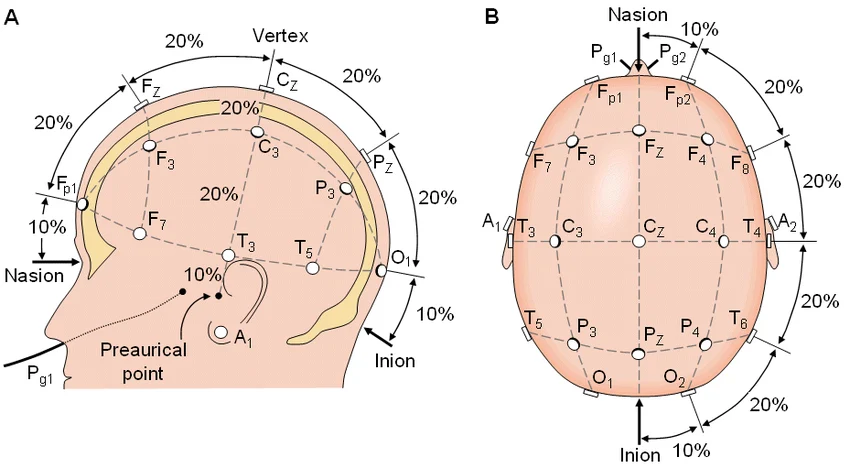
\includegraphics[width=0.86\textwidth]{../memoria/figs/sistema_10_20.png}

            \vspace{0.1cm}
            {\scriptsize Sistema internacional 10--20}
        \end{column}
    \end{columns}
\end{frame}

\begin{frame}{Señal por canales}
    \centering
    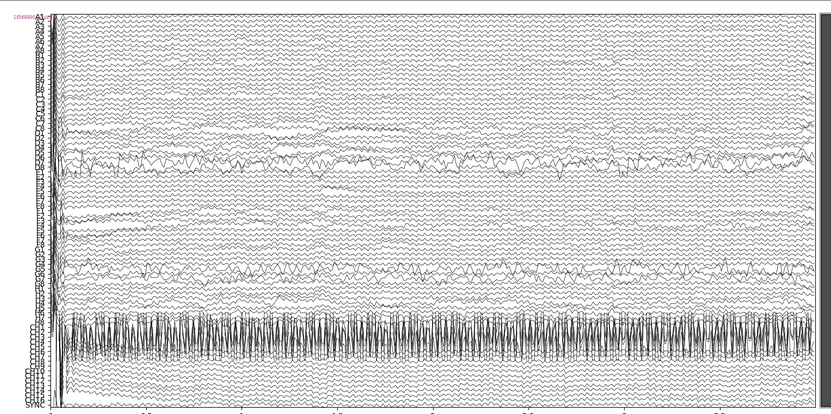
\includegraphics[width=0.82\textwidth]{figs/channels.png}

    \vspace{0.25cm}
    \begin{center}
        {\small Cada canal registra una señal temporal distinta, asociada a una posición del montaje.}
    \end{center}
\end{frame}

\begin{frame}{Motivación}
    \begin{columns}[c,onlytextwidth]
        \begin{column}{0.38\textwidth}
            \begin{tikzpicture}[
                motivo/.style={
                    rectangle,
                    rounded corners=3pt,
                    fill=urjcred!8,
                    draw=urjcred!35,
                    text width=4.0cm,
                    minimum height=1.0cm,
                    align=left,
                    font=\small,
                    inner xsep=8pt
                }
            ]
                \node[motivo] (a) {\textbf{Prueba del sueño}\\Primer contacto con señales EEG};
                \node[motivo, below=0.4cm of a] (b) {\textbf{Pregunta}\\¿Puede un modelo de IA entender estas señales?};
            \end{tikzpicture}
        \end{column}

        \begin{column}{0.58\textwidth}
            \centering
            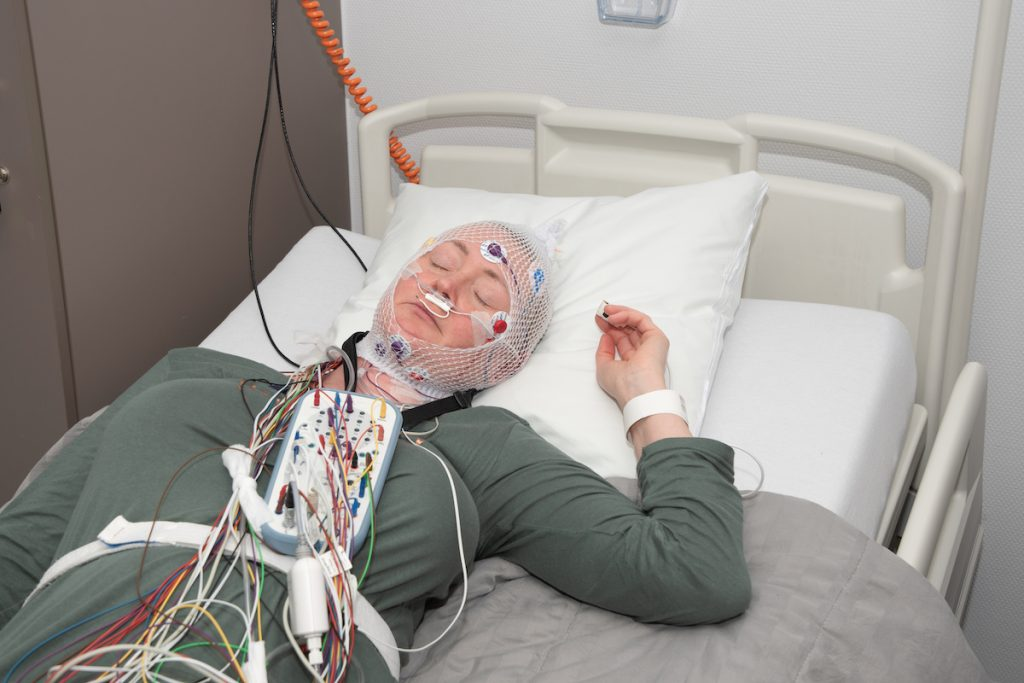
\includegraphics[width=0.92\textwidth]{figs/prueba_sueno.png}
        \end{column}
    \end{columns}
\end{frame}

\begin{frame}{Más allá de lo observable}
    \centering
    \begin{tikzpicture}[
        header/.style={
            rectangle,
            rounded corners=5pt,
            fill=urjcred!8,
            draw=urjcred!38,
            text width=10.2cm,
            minimum height=0.72cm,
            align=center,
            font=\small\bfseries
        },
        pista/.style={
            rectangle,
            rounded corners=5pt,
            fill=black!5,
            draw=black!24,
            text width=3.15cm,
            minimum height=0.78cm,
            align=center,
            font=\small
        },
        caso/.style={
            rectangle,
            rounded corners=5pt,
            fill=softblue!9,
            draw=softblue!38,
            text width=3.15cm,
            minimum height=0.82cm,
            align=center,
            font=\scriptsize
        },
        cierre/.style={
            rectangle,
            rounded corners=6pt,
            fill=softgreen!13,
            draw=softgreen!45,
            text width=7.1cm,
            minimum height=0.86cm,
            align=center,
            font=\small\bfseries
        }
    ]
        \node[header] at (0,2.35) {¿Cómo reconocemos normalmente una emoción?};
        \node[pista] at (-3.85,1.38) {Voz y palabras};
        \node[pista] at (0,1.38) {Gestos};
        \node[pista] at (3.85,1.38) {Expresión facial};

        \node[header] at (0,0.18) {Hay situaciones en las que eso no basta};
        \node[caso] at (-3.85,-0.82) {dificultades\\de comunicación};
        \node[caso] at (0,-0.82) {expresión\\reducida};
        \node[caso] at (3.85,-0.82) {contexto\\médico};

        \draw[-{Latex[length=2.2mm]}, thick, draw=black!45] (0,-1.38) -- (0,-1.78);
        \node[cierre] at (0,-2.28) {Señales EEG para reconocer emociones};
    \end{tikzpicture}
\end{frame}

\begin{frame}{¿Por qué IA explicable?}
    \begin{columns}[c,onlytextwidth]
        \begin{column}{0.64\textwidth}
            \begin{beamercolorbox}[rounded=true,sep=0.18cm,wd=\textwidth,center]{block body}
                {\small\bfseries Modelo explicable}

                \vspace{0.15cm}
                \begin{columns}[c,onlytextwidth]
                    \begin{column}{0.28\textwidth}
                        \centering
                        
\includegraphics[height=1.95cm]{figs/akinator.png}
                    \end{column}
                    \begin{column}{0.68\textwidth}
                        \centering
                        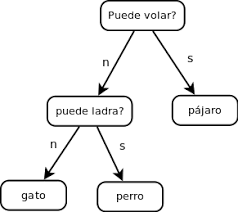
\includegraphics[width=\textwidth]{../memoria/figs/Arbol_decision.png}
                    \end{column}
                \end{columns}

                \vspace{0.18cm}
                \begin{tikzpicture}
                    \node[
                        rectangle,
                        rounded corners=3pt,
                        fill=softgreen!12,
                        draw=softgreen!45,
                        text width=6.4cm,
                        align=center,
                        minimum height=0.62cm,
                        font=\scriptsize
                    ] {Preguntas sucesivas hasta llegar a una decisión};
                \end{tikzpicture}
            \end{beamercolorbox}
        \end{column}

        \begin{column}{0.33\textwidth}
            \begin{beamercolorbox}[rounded=true,sep=0.18cm,wd=\textwidth,center]{block body}
                {\small\bfseries Caja negra}

                \vspace{0.22cm}
                
\includegraphics[height=1.75cm]{figs/chatgpt.png}

                \vspace{0.35cm}
                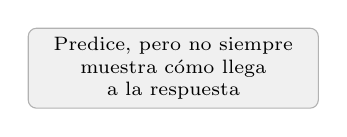
\begin{tikzpicture}
                    \node[
                        rectangle,
                        rounded corners=3pt,
                        fill=black!6,
                        draw=black!30,
                        text width=3.45cm,
                        align=center,
                        minimum height=0.95cm,
                        font=\scriptsize
                    ] {Predice, pero no siempre\\muestra cómo llega\\a la respuesta};
                \end{tikzpicture}
            \end{beamercolorbox}
        \end{column}
    \end{columns}

    \vspace{0.38cm}
    {\small En aplicaciones médicas, acertar no es suficiente: también hay que justificar la decisión.}
\end{frame}

\begin{frame}{Emociones analizadas}
    \centering
    \vspace{0.15cm}
    \begin{tikzpicture}[
        emocion/.style={
            rectangle,
            rounded corners=5pt,
            minimum width=3.35cm,
            minimum height=2.1cm,
            align=center,
            font=\small,
            draw=black!25,
            line width=0.5pt
        }
    ]
        \node[emocion, fill=red!16, draw=red!35] (joy) {
            {\Large\bfseries JOY}\\[2mm]
            respuesta positiva
        };
        \node[emocion, fill=green!16, draw=green!35!black, right=0.55cm of joy] (neutro) {
            {\Large\bfseries NEUTRO}\\[2mm]
            estado de referencia
        };
        \node[emocion, fill=blue!14, draw=blue!35, right=0.55cm of neutro] (sad) {
            {\Large\bfseries SAD}\\[2mm]
            respuesta negativa
        };
    \end{tikzpicture}

    \vspace{0.55cm}
    \begin{tikzpicture}
        \node[
            rectangle,
            rounded corners=3pt,
            fill=urjcred!8,
            draw=urjcred!35,
            text width=9.4cm,
            align=center,
            minimum height=0.9cm,
            font=\small
        ] {Tres clases simples para comprobar si el sistema distingue cambios emocionales respecto a una condición neutra.};
    \end{tikzpicture}
\end{frame}
